L'odierna rete elettrica è stata progettata come un sistema centralizzato, in cui l'energia elettrica fluisce attraverso linee unidirezionali di trasmissione e distribuzione dai generatori fino ai clienti finali. La logica applicativa è concentrata in zona centrale e solo parzialmente nelle \emph{substation}, mentre le componenti restanti sono quasi totalmente passive. Una Smart Grid, mostrata dal punto di vista strutturale in figura \ref{fig:1}, fornisce una più elevata ed ampia intelligenza distribuita incorporata nei dispositivi locali, comunicazione e scambio bidirezionale di informazioni ed elettricità.

\begin{figure}[h] \centering{
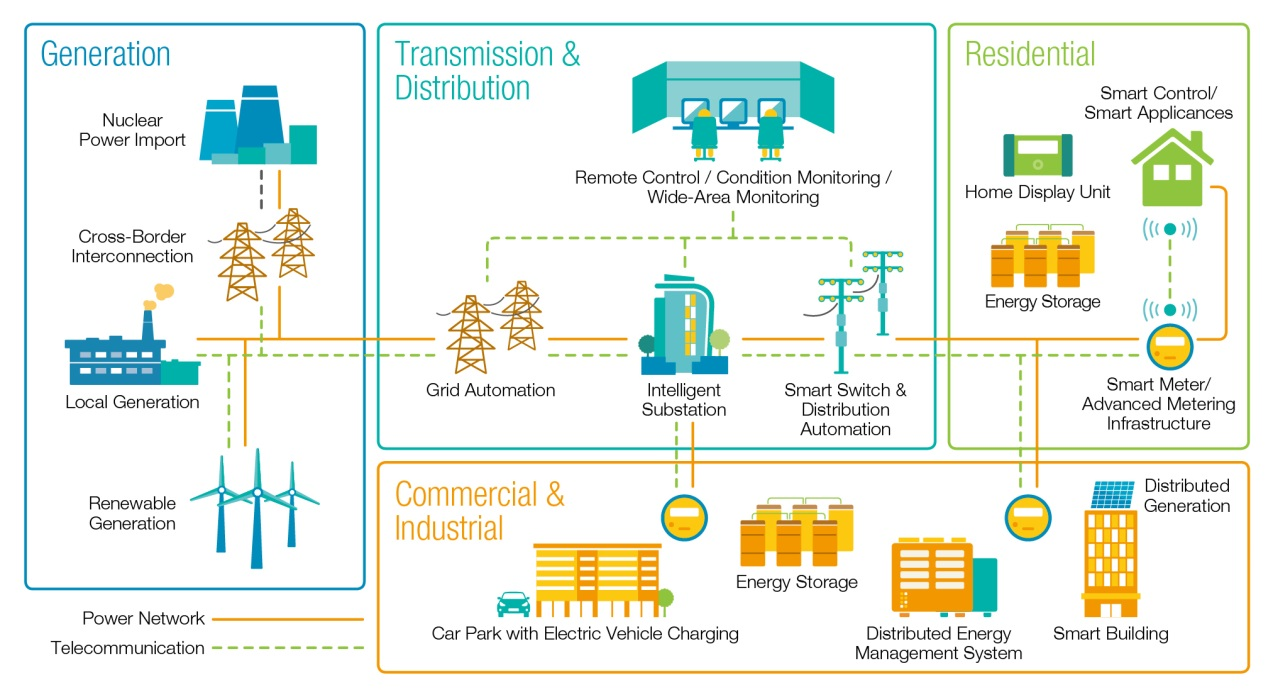
\includegraphics[scale=0.95]{imgs/architecture.jpg}}
\caption{Smart Grid}\label{fig:1}
\end{figure}

\section{Smart Grid Framework}
Le Smart Grid richiedono sia una complessa infrastruttura di comunicazione, che sofisticate tecnologie di comunicazione e computazione. Entrambe consentono la conservazione di parte dell'energia prodotta e l'introduzione di nuovi metodi di gestione della domanda energetica, per adottare politiche di bilanciamento del carico, controllare instabilità energetiche causate dalla natura delle risorse rinnovabili e prevenire la diffusione di fallimenti in cascata nella rete. 
\newline 
La figura \ref{fig:2} riassume le principali tematiche relative alle Smart Grid:
\begin{itemize}
	\item \emph{Energy infrastructure} rappresenta la base fisica ed organizzativa necessaria per la generazione, trasmissione e distribuzione dell'energia;
	\item \emph{Communication infrastructure} è responsabile del trasferimento di informazioni critiche attraverso la rete;
	\item \emph{Information technology} fornisce modelli, analisi, visualizzazioni web e transazioni commerciali;
	\item \emph{Potential applications} offre tecniche di generazione, gestione, automatizzazione e rilevamento per l'intero sistema.
\end{itemize} 

\begin{figure}[h] \centering{
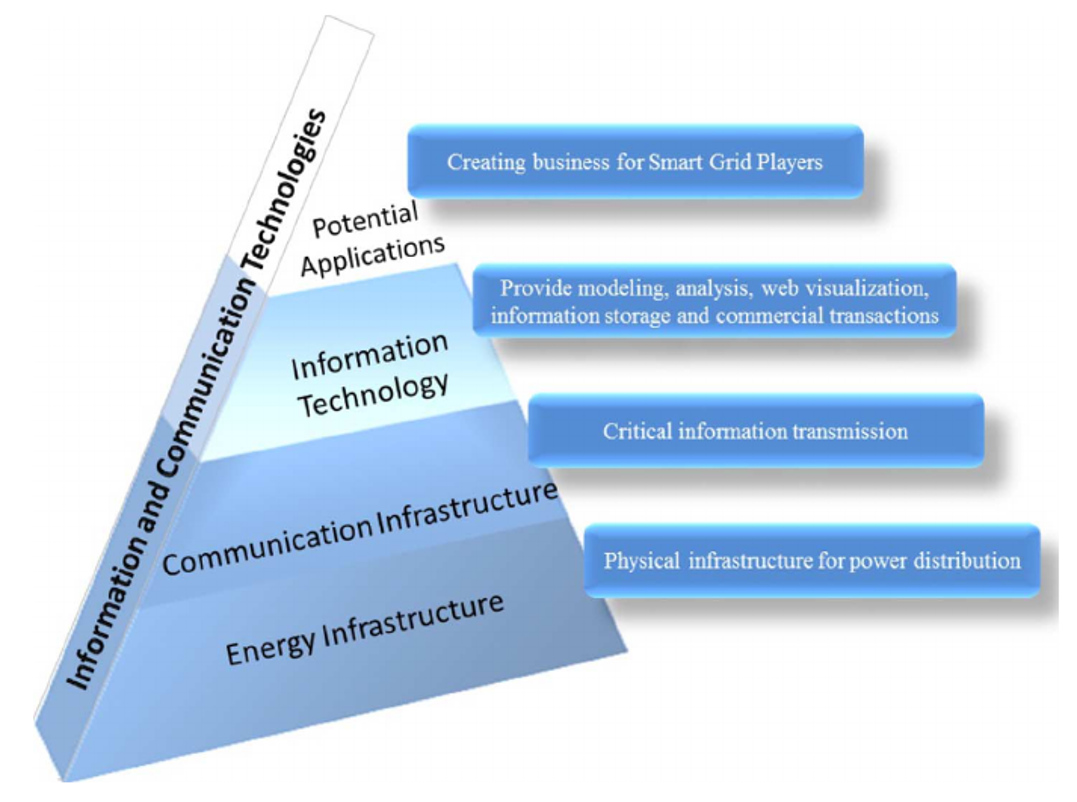
\includegraphics[scale=0.3, natwidth=1003,natheight=490]{imgs/ict.png}}
\caption{Smart Grid framework}\label{fig:2}
\end{figure}

La communication infrastructure svolge un ruolo cruciale, ossia collegare tutte le componenti della rete collezionando informazioni sulle loro condizioni, per scopi di controllo, monitoraggio e manutenzione. Eventuali problemi legati all'energy instrastructure possono essere evitati se corrette operazioni vengono prese con l'aiuto della communication infrastructure. 
\newline 
Differenti tecnologie di comunicazione posso essere usate per diversi scopi e requisiti in base all'applicazione. L'information technology fornisce una piattaforma comune di scambio di informazioni proveniente da differenti attività legate alla Smart Grid, che permette l'integrazione di informazioni da diversi livelli, dando sostegno alla raccolta di diverse informazioni, all'analisi e ad applicazioni avanzate.
\newline
Le tecniche dell'applications layer generalmente mirano a ridurre il consumo energetico dei clienti, cambiando i loro comportamenti di consumo, dotandoli di strumenti di monitoraggio.    
\newline
La figura \ref{fig:3} mostra le componenti della Smart Grid, illustrate dall'energy infrastructure al potentional applications.

\begin{figure}[h] \centering{
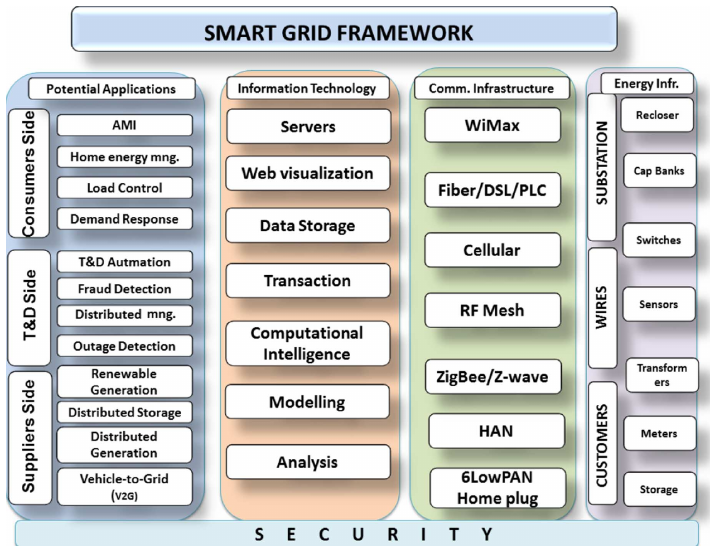
\includegraphics[scale=0.7, natwidth=1003,natheight=490]{imgs/sgframework.png}}
\caption{Smart Grid framework}\label{fig:3}
\end{figure}

%\section{Communication architecture}
\newpage
Il concetto di Smart Grid mira a realizzare un sofisticato sistema, integrando information technology e communication infrastructure all'attuale sistema di alimentazione e il nuovo sistema di generazione distribuito, in modo da sfruttare pienamente l'uso di risorse rinnovabili e di massimizzare l'efficienza energetica. Da una prospettiva leggermente diversa, una Smart Grid può essere considerata come una rete di comunicazione di dati che riesce, grazie al supporto di specifici dispositivi di gestione dell'energia, a far collaborare le diverse componenti della rete in maniera flessibile e senza discontinuità, per un utilizzo efficiente dell'energia.
%\newline
%L'architettura \emph{end-to-end} delle Smart Grid (fig. \ref{fig:4}) fondamentalmente comprendono tre livelli principali:
%\begin{itemize}
%	\item \emph{Application layer}, include applicazioni avanzate fornendo interoperabilità fra di esse; si occupa principalmente della gestione della domanda/risposta, interruzioni, infrastruttura di metering, delle risose ed rilevamento di frodi;
%	\item \emph{Power layer}, comprende i sistemi di generazione, trasmissione e distribuzione, l'integrazione di risorse rinnovabili ed il sistema di comunicazione bidirezionale;  
%	\item \emph{Communication layer}, rappresenta il cuore del sistema fornendo la connettività fra tutte le parti e dispositivi di esso. 
%\end{itemize}     

%\begin{figure}[h] \centering{
%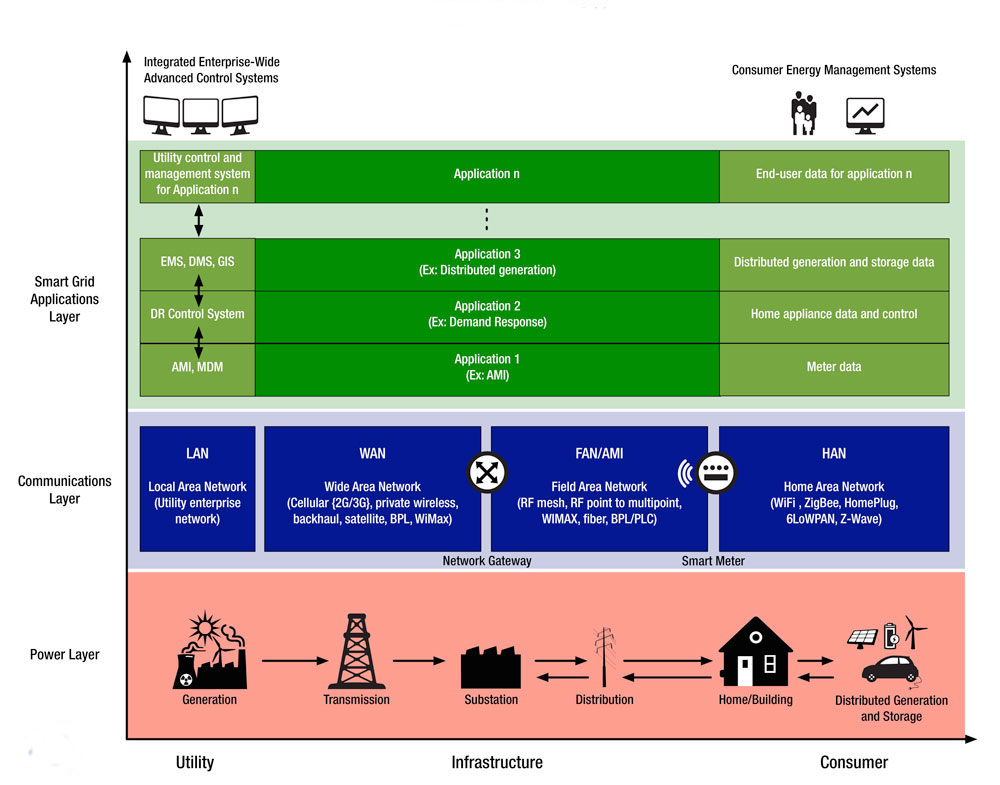
\includegraphics[scale=0.4, natwidth=1003,natheight=490]{imgs/endtoendtax.jpg}}
%\caption{Architettura end-to-end}\label{fig:4}
%\end{figure}

La comunicazione consiste di tre categorie di trasmissione, con relativi standard e protocolli (vedi cap.):
\begin{itemize}
	\item \emph{Wide-area network} (WAN);
	\item \emph{Field-area network} (FAN);
	\item \emph{Home-area network} (HAN).
\end{itemize}

%Il communication layer consiste di tre categorie di trasmissione:
%\begin{itemize}
%	\item \emph{Wide-area network} (WAN);
%	\item \emph{Field-area network} (FAN);
%	\item \emph{Home-area network} (HAN).
%\end{itemize}

\subsection{Wide-area network}
La WAN consente la comunicazione fra le entità che forniscono energia e le substations; deve estendersi su tutte le substation, strutture di distribuzione, generazione energetica e di conservazione dell'energia, per poter essere efficace e scalabile. Essa è rete di comunicazione bidirezionale ad alta larghezza di banda che gestisce le trasmissioni a lunga distanza dei dati con avanzate applicazioni di misurazione e monitoraggio. La comunicazione remota fra le \emph{utility} e gli smart meter è essenziale per lo scambio di importanti informazioni, quali prezzi e tariffe dei clienti. Le reti cellulari, WiMAX e comunicazioni cablate, in particolare comunicazioni basate su fibra ottica e microwave, sono i migliori candidati come tecnlogie per WAN (vedi cap. 4).
\newline
Il sistema di distribuzione agisce da punto di aggregazione fra FAN e WAN, come ad esempio una substation o una torre di comunicazione che colleziona tutte le informazioni prodotte dagli smart meter e le trasferisce alla rete di comunicazione principale. Oltre che da punto di aggregazione tali dispositivi possono fungere da punti di conservazione dell'energia per eventuali interruzioni o guasti.

\subsection{Field-area network}
La FAN può essere descritta come una rete di comunicazione per aree di distribuzione dell'energia e che mette in contatto l'automazione della distribuzione e dispositivi di controllo alle sedi dei consumatori. Essa agisce, quindi, come un intermediario fra le substation e le sedi dei clienti, con nodi intelligenti in grado di raccogliere e controllare i dati da remoto. Tali nodi sono connessi ad un gateway centralizzato, il quale è alimentato costantemente in modo da poter trasmettere i dati raccolti. I canali a bassa larghezza di banda della FAN sono altamente robusti per la trasmissione affidabile di dati. 
\newline 
La scelta delle tecnologie di comunicazione  variano per la FAN in base alle esigenze della Smart Grid: fibra ottica per avere bassa latenza e perfomance di comunicazione superiori, oppure WiMAX se le reti cellulari non riescono a coprire l'area di interesse, ma l'attuale orientamento ricade sull'utilizzo dello standard IEC 61850 (vedi cap. ), il quale fornisce interoperabilità e comunicazione fra i dispositivi elettronici intelligenti.

\subsection{Home-area network}{
Gli smart meter riescono a connettersi alla HAN, in modo tale che i consumatori siano in grado di conoscere l'importo da pagare e gestire il loro consumo ed avere il controllo dei propri elettrodomestici intelligenti, attraverso display presenti in casa e interfacce web. 
\newline 
Le migliori tecnologie di comunicazione per HAN sono ZigBee,Wi-Fi, HomePlug, Z-wave e M-Bus (vedi cap.).
}

\vspace{20pt}\hspace{-17pt}Nelle sezioni successive vengono presentate le tecnologie e le infrastrutture abilitanti di una Smart Grid, a partire dalla generazione e conservazione dell'energia fino ad arrivare alla trasmissione e distribuzione.

\section{Generazione di energia rinnovabile}
Le risorse di energia rinnovabile sono state sviluppate in molti paesi per ridurre l'inquinamento e fornire energia elettrica sostenibile. A differenza delle tradizionali fonti di energia, le quali creano inquinamento, le risorse di energia rinnovabile non esauriscono risorse naturali nel processo di creazione di energia e sono adattabili ovunque, in base alle dimensioni a partire dall'applicazione su una singola casa fino a dimensioni su larga scala.
\newline
Le più comuni risorse di energia rinnovabile sono:
\begin{itemize}
	\item \emph{Sistemi fotovoltaici}, i quali convertono l'energia solare direttamente in elettricità, attraverso pannelli solari esposti al sole. Tali pannelli sono costituiti da celle solari che contengono materiale fotovoltaico, le quali trasmettono elettroni tra diverse bande all'interno del materiale generando differenza di potenziale fra due elettrodi, che consente alla corrente continua di fluire;
	\item \emph{Sistemi per l'energia solare termica}, che convertono energia solare in calore. Esistono tre tipi di raccoglitori in base alla temperatura, da bassa per riscaldare piccoli spazi ad alta per l'utilizzo nella produzione di energia elettrica;
	\item \emph{Vento}, la cui energia viene convertita tramite turbine in elettricità. Il principale aspetto negativo deriva dall'intermittenza del vento, specularmente per i sistemi basati sull'energia solare;
	\item \emph{Biomasse}, ovvero la produzione di elettricità a partire da elementi naturali morti, anche se questa causa inquinamento atmosferico;
	\item \emph{Sistemi che sfruttano la potenza dell'acqua}, sia che essa sia generata artificialmente che naturalmente, grazie alle onde e alle maree.   
\end{itemize} 

 
\section{Conservazione dell'energia}

\section{Veicoli elettrici}

\section{Microgrid}



\section{Smart substation}

\subsection{IED}
\subsection{Sensor}
\subsection{SCADA}



\section{Sistemi di trasmissione}

\subsection{Sistemi di gestione dell'energia}
\subsection{FACTS}
\subsection{HVDC}
\subsection{WAMPAC}


\section{Sistemi di distribuzione}

\subsection{Sistemi di gestione della distribuzione}
\subsubsection{distribution SCADA}
\subsection{Volt/VAr control}


%
%\subsection{smart substation} 3.3 , 3.3.8 role
%IED, sensor, scada, RTU, 
%
%\subsection{energy storage}
%veicoli, microgrid (3.2.4)
%
%\subsection{generazione di energia da risorse rinnovabili}
%
%\subsection{trasmission systems} 3.4 (pag.154) role 209
%facts hdvc 3.4.2 (pag.168), WAMPC 3.4.3 (pag.187) 202 role
%
%\subsection{distribution systems} 3.5 pag.211
%distribution scada, Fault Detection, Isolation, and Service Restoration 244, componenti, outage management
%
%\subsection{communication systems} 265
%ami, 
%
%\subsection{monitoring and diagnostics}
%
%\subsection{SMART METERS AND ADVANCED METERING INFRASTRUCTURE}
%
%vedere anche 3.4.1.4 



% http://ieeexplore.ieee.org/stamp/stamp.jsp?tp=&arnumber=6298960 

%http://www.smartgridinformation.info/pdf/5264_doc_1.pdf

% http://www.cs.nmsu.edu/~misra/papers/SmartGridSurvey.pdf


%libri 

